\documentclass{article} % For LaTeX2e
\usepackage{nips15submit_e,times}
\usepackage{hyperref}
\usepackage{url}
\usepackage{enumerate}
\usepackage{graphicx} 
\usepackage{caption}
\usepackage{subcaption}
%\usepackage{subfigure}
\usepackage{amsmath}
%\documentstyle[nips14submit_09,times,art10]{article} % For LaTeX 2.09


\title{Report - Autonomous Driving: Object Detection}


\author{
Zhen Li \\
Department of Computer Science\\
University of Toronto\\
Toronto, ON, M5S 2E4 \\
\href{mailto:zhen@cs.toronto.edu}{\texttt{zhen@cs.toronto.edu}}
\And
Zhicong Lu \\
Department of Computer Science\\
University of Toronto\\
Toronto, ON, M5S 2E4 \\
\href{mailto:luzhc@cs.toronto.edu}{\texttt{luzhc@cs.toronto.edu}}
}

% The \author macro works with any number of authors. There are two commands
% used to separate the names and addresses of multiple authors: \And and \AND.
%
% Using \And between authors leaves it to \LaTeX{} to determine where to break
% the lines. Using \AND forces a linebreak at that point. So, if \LaTeX{}
% puts 3 of 4 authors names on the first line, and the last on the second
% line, try using \AND instead of \And before the third author name.

\newcommand{\fix}{\marginpar{FIX}}
\newcommand{\new}{\marginpar{NEW}}

%\nipsfinalcopy % Uncomment for camera-ready version

\begin{document}


\maketitle

\iffalse
\begin{abstract}
TODO: The abstract paragraph should be indented 1/2~inch (3~picas) on both left and
right-hand margins. Use 10~point type, with a vertical spacing of 11~points.
The word \textbf{Abstract} must be centered, bold, and in point size 12. Two
line spaces precede the abstract. The abstract must be limited to one
paragraph.
\end{abstract}
\fi

\section{Introduction}

Object detection has always been one of the core problems of Computer Vision and Machine Learning. Based on object detection, autonomous driving has become the most challenging topic in this field which has a great impact on our life. The goal of this project is to detect the cars and pedestrians in the real road images, and locate the 2D bounding boxes of the objects correctly. Such detection techniques would make vision-based autonomous driving systems more robust and accurate, hence increasing the possibility of adopting them in the real life. 

It is hard to apply classical machine learning techniques on this topic directly. Compared with the traditional object recognition database, for example, the MNIST Database \cite{lecun1998gradient}, the real road images have more occlusions, more complicated background textures, and as a result, objects from the real road images are harder to detect. 

The basic idea of this project came from The KITTI Vision Benchmark Suite \cite{Geiger2012CVPR}. It provides a well labeled training set containing $7481$ color images, including several classes such as cars, pedestrians, cyclists, vans, trucks, etc. Inspired by the ranking of different methods on the KITTI website, we would try to implement those with very good performance and without using other sensor data (or dual camera information), for the reason that such methods are more accessible and have better potential to be implemented even on mobile devices. We would try to improve the training model based on the findings of the state-of-the-art to come up with our own method, and evaluate the performance of it. We expect that our method can reach a high accuracy on the test set with an optimized speed. 

In this project, we focus on the performance of SVM, Regionlets \cite{Wang2013}, and CNN techniques as well as their differences. Our code is available on GitHub\footnote{https://github.com/CommanderLee/ObjectDetection}.

\section{Related work}

The object detection, especially cars and pedestrians detection for the autonomous driving system, has been a hot topic in computer vision for recent years. In many tasks, since the number of images and windows to evaluate is huge, we often rely on a weak classifier to get proposals for the more expensive classifier. Selective Search \cite{van2011segmentation} is a successful algorithm, which emphasize recall to include all image fragments of potential relevance. It can be combined with many feature representation techniques, such as the histograms of oriented gradients (HOG) \cite{dalal2005histograms}, and SIFT \cite{lowe2004distinctive}. 

[TODO: introduce Regionlets]

Convolutional Neural Network (CNN or ConvNet) \cite{Krizhevsky2012} is able to learn the features of the object and handle variations such as poses, viewpoints, and light conditions, with high accuracy and high efficiency. However, it doesn't perform well when occlusion occurs, which is often the case in pedestrian and cyclists detection. 

Recently, the Fully Convolutional Neural Network (FCN) based methods[5], with end-to-end approach of learning model parameters and image features, further improves the performance of object detection. DenseBox \cite{Huang2015} is a unified end-to-end FCN that
directly predicts bounding boxes and object class confidences through all locations
and scales of an image with great accuracy and efficiency. It also incorporates with landmark localization during multitask learning and further improves
object detection accuracy. It has the best accuracy on car detection on KITTI by the time the proposal is finished. However, it has not been tested on the tasks of pedestrian or cyclists detection.

Felzenszwalb et al \cite{felzenszwalb2010object} combined a margin-sensitive approach for data-mining hard negative samples, which can be used by iteratively adding hard negative examples (false positive errors) \cite{van2011segmentation}.

\section{Methods}

\subsection{Object detection system}


\begin{figure}[htb]
\begin{subfigure}[b]{0.9\textwidth}
    \centering
    \includegraphics[width=.9\linewidth]{pipeline1.png}
    \label{fig:pipeline1}
\end{subfigure}
\begin{subfigure}[b]{0.9\textwidth}
    \centering
    \includegraphics[width=.9\linewidth]{pipeline2.png}
    \label{fig:pipeline2}
\end{subfigure}
\caption{Top: The pipeline for training procedure. Bottom: The pipeline for testing procedure.
\label{fig:pipeline}}
\end{figure}


The whole architecture of our detection system is illustrated in Figure \ref{fig:pipeline}. In the training procedure, cropped images with ground truth labels are utilized to train the initial model. After validation, false positive errors are added to the negative samples, which iteratively emphasize the hard cases. 

In the testing procedure, there are mainly three steps: 
\begin{enumerate}[Step 1]
    \item Weak classifier: Generate proposals and save the bounding box.
    \item Extract features: Calculate feature matrix from the cropped image box.
    \item Strong classifier: Find out cars and pedestrians, and save the results.
\end{enumerate}

We use the Selective Search \cite{van2011segmentation} as the common weak classifier. For the strong classifier after it, we use SVM, Regionlets, and CNN.

\subsection{Image multiplication for ground truth generation}
\label{sec:positive}

In training, image segments of cars and pedestrians are cropped and resized to $64 \times 64$, according to the corresponding labels. Then we adjust the original image by adding a random bias to the histogram map (from $-20\%$ to $+20\%$) repeatedly. We also reverse the original image horizontally to make full use of the training set. This adjustment will not only balance the different light conditions in the original images, but also make full use of the hidden information. 

\subsection{Selective Search for negative samples generation}

We use the Selective Search \cite{van2011segmentation} to generate the negative samples. Selective Search is a segmentation algorithm that focus on recall rate and ensure its results do not stem from parameter tuning. It starts from initial regions generated by \cite{felzenszwalb2004efficient}, and use a greedy algorithm to repeatedly merge similar segments. The similarity function is defined to combine the size similarity, by calculating the fraction of joint area, and the texture similarity, by calculating the histogram intersection.

We randomly select images from the training set, run Selective Search, and find out background segments, which are defined to have a $0\%$ to $30\%$ overlap with a positive sample (car or pedestrian). We generated $20000$ negative samples for training. 

\subsection{Retrain procedure}

Generating the negative samples is a important part of road object detection, since the background textures are too complicated to cluster easily. Too enhance the model's ability to solve hard problems, we add retrain procedure \cite{felzenszwalb2010object} to iteratively adding false positive errors to the negative sample set.


\subsection{Regionlets with Adaboost for generic object detection}

To try some different features as well as different classifiers, we implemented Regionlets \cite{Wang2013} for generic object detection to compare with the SVM classifier. We also use Selective Search \cite{van2011segmentation} to get candidate bounding boxes which may contain target object, and classify the candidate boxes with the boosted classifiers.


\begin{figure}[htb]
	\centering
	\includegraphics[width=6cm]{regionlets_def.png}
	\caption{Illustration of Regionlets definition}
	\label{fig:regionlet_def}
\end{figure}


\subsubsection{Regionlet definition}

Regionlets are defined as sub-parts of a region in the image. They are introduced to act as basic units to extract appearance features, and are organized into small groups to describe features with different degrees of deformation \cite{Wang2013}. In this way, features extracted from small regions and a big region can work together, which can provide a good localization ability as well as tolerate more variations.

Figure \ref{fig:regionlet_def} shows the definition of regionlets. The outer black rectangle is a candidate bounding box. The blue rectangle inside the bounding box is a feature extraction region denoted as $R$, which will contribute a weak classifier to the boosting classifier. Within the region $R$, some small sub-regions are selected and defined as a group of regionlets, as shown in Figure \ref{fig:regionlet_def}. The features of these regionlets will be aggregated to a single feature for a region $R$ during training, and a bounding box will be represented by a number of such regions.

By introducing regionlets, it is straightforward to think that it would improve object recognition especially for occluded situations, which are common in automated driving, because the discerning features are extracted while irrelevant appearance from background is largely discarded. Besides, more regionlets in a single region $R$ will increase the capacity to model deformations.


\subsubsection{Regionlet feature extraction}

According to \cite{Wang2013}, feature extraction from $R$ takes 2 steps. First, we extract appearance features of HOG descriptors \cite{dalal2005histograms} from each regionlets respectively. Second, we generate the representation of R based on regionlet’s features. We apply max-pooling over regionlet features for the feature of region $R$. Denote $T(R)$ as the feature representation for region $R$, $T(r_j)$ as the feature extracted from the $jth$ region $r_j$ in $R$, then the operation is defined as follows:

\begin{equation}
T(R) = \max \limits_j T(r_j)
\end{equation}

The max-pooling happens for each feature dimension independently. For each regionlet, we first extract HOG feature for the regionlet. Then we pick a 1D feature from the same dimension of HOG feature in each regionlet and apply max-pooling to get the feature for region R. We have millions of such 1D features in a detection window and the most discriminative ones are determined through a boosting learning process.

\subsubsection{Training with boosting regionlet features}
\label{training_regionlets}

We use the ensemble method of boosting to learn the discriminative regionlet groups and their configurations from a huge pool of candidate regions and regionlets.

To deal with deformation at different scales, we first build a largely over-complete pool for regions and regionlets with various positions, aspect ratios and sizes, as in \cite{Wang2013}. 
We denote the 1D feature of a region relative to a bounding box as $R'= (l', t', r', b', k)$, where $k$ denotes the $k$-th element of the low-level feature vector (HOG features) of the region. The region pool is spanned by $X \times Y \times W \times H \times F$, where $X$ and $Y$ are respectively the space of horizontal and vertical position of region $R'$ in the detection window, $W$ and $H$ are the width and height of the region $R'$, and $F$ is the space of HOG feature. Enumerating all possible regions is impractical and not necessary. We employ a sampling process to reduce the pool size. The algorithm is the same as Algorithm 1 in \cite{Wang2013}.

After getting the region pool, we propose a set of regionlets with random positions inside each region. Although the sizes of regionlets in a region could be arbitrary in general, we restrict regionlets in a group to have the identical size because the regionlets are designed to capture the same appearance in different possible locations due to deformation\cite{Wang2013}. The sizes of regionlets in different groups could be different. A region contains 5 regionlets in our implementation.

The final feature space used as the feature pool for boosting is spanned by $R \times C$, where $R$ is the region feature prototype space and $C$ is the configuration space of regionlets.

We use Gentle Adaboost \cite{Torralba04sharingfeatures:} to train classifiers for our object detector. One boosting classifier consists of a set of selected weak classifiers. We define the weak classifier as a decision tree. Gentle Adaboost puts less weight on outlier data points, which would make the classifiers more robust.

\section{Experiments}

\subsection{Data set}

We use the KITTI data set for Object Detection \cite{Geiger2012CVPR}, which contains $7481$ color images with ground truth bounding box labels, including $28782$ cars and $4487$ pedestrians. We partition the data set to a training set contains $5237$ images ($70\%$), and a testing set contains $2244$ images ($30\%$). Then we run different algorithms on the data set and analyze the results.

\subsection{SVM}

\subsubsection{Training}

We noticed that there are far more cars than pedestrians in the KITTI data set. To balance the difference, the multiplication trick in Section \ref{sec:positive} can be used to increase the number of pedestrians, which makes better use of the training set. In addition, since the KITTI benchmark only evaluate objects larger than $25$ pixels (height), we ignore these small objects in the training set. After all of these augmenting and filtering strategies, we have $22576$ cars and $20960$ pedestrians as positive samples for training.

The SVM classifier is trained with the cropped positive samples with ground truth labels, and negative background segments generated by the Selective Search. Since SVM is a binary classifier, we trained 3 classifiers: (1) Car vs All, (2) Pedestrian vs All, and (3) Car vs Pedestrian. We use the \texttt{fitcsvm} function from the MATLAB toolbox to train out model.

\begin{figure}[htb]
\begin{center}
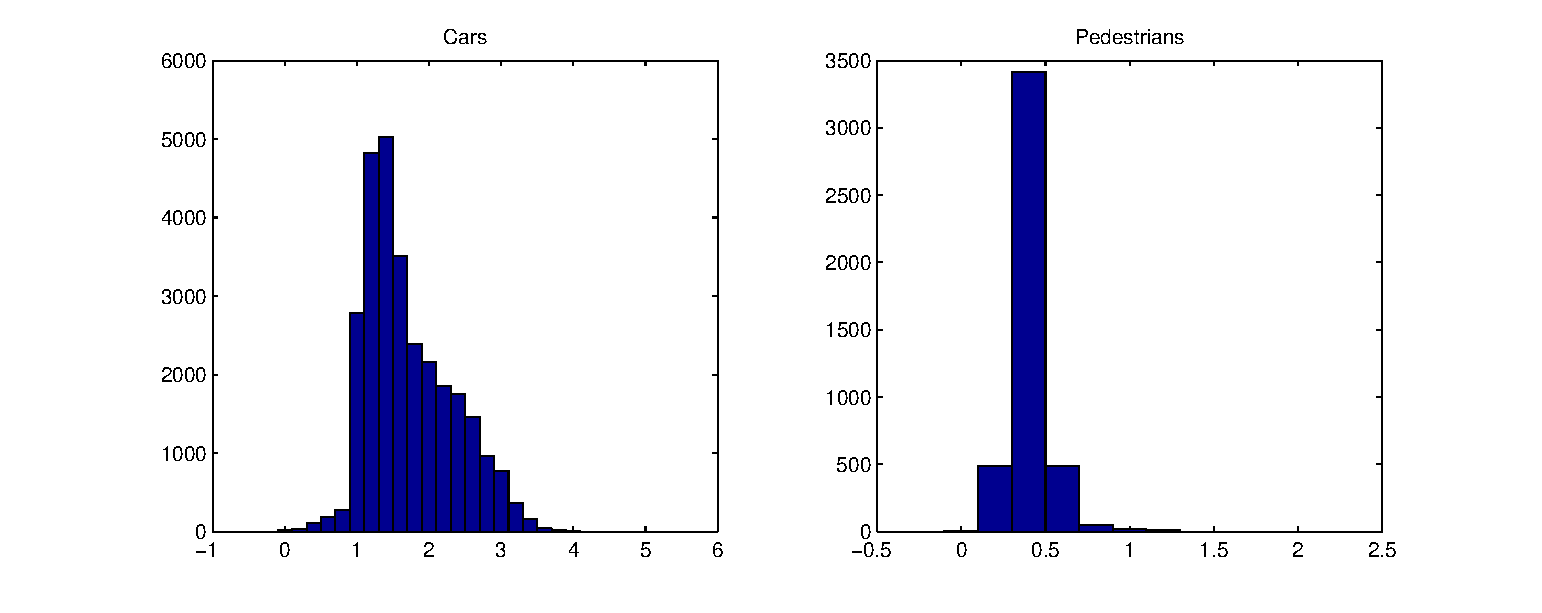
\includegraphics[width=\textwidth]{aspect_ratio.eps}
\end{center}
\caption{Normalized aspect ratio (width/height) distributions on segments of cropped cars and pedestrians.
\label{fig:aspect_ratio}}
\end{figure}

As illustrated in Figure \ref{fig:pipeline}, there are 3 steps in our detector: (1) Generate proposals with Selective Search, (2) Extract HOG features, and (3) Predict with a SVM classifier. Since the last two steps are relatively expensive, we add some filters to remove the irrelevant proposals after step (1). First, we can remove the small objects (height less than 25 pixels) according to the requirement of KITTI benchmark. Second, according to the distribution of the aspect ratio of cars and pedestrians in Figure \ref{fig:aspect_ratio}, we can early stop the proposal segments which are obviously not cars or pedestrians.

\subsubsection{Validation}

We use the k-fold ($k=7$) cross validation to evaluate our model, as required by the project guide ($60\%$ training, $10\%$ validation, and $30\%$ testing). According to our description in Section \ref{sec:positive}, we multiply the data set by changing the contrast and brightness of the images, as well as reversing the images horizontally. Then we can compare the cross loss before and after the multiplication, using the \texttt{crossval} function from the MATLAB toolbox.


\begin{figure}[htb]
\begin{center}
%\framebox[4.0in]{crossloss.eps}
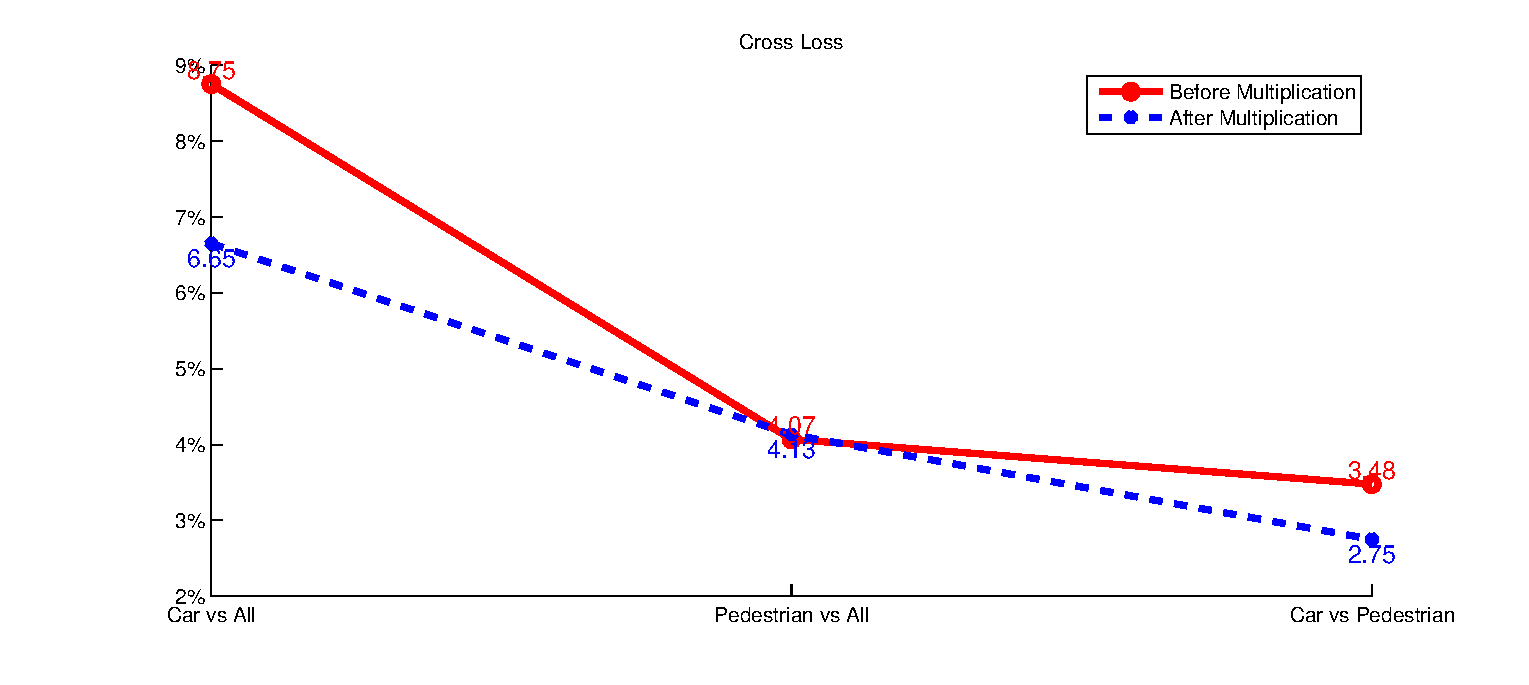
\includegraphics[width=.8\textwidth]{crossloss.eps}
%\fbox{\rule[-.5cm]{0cm}{4cm} \rule[-.5cm]{4cm}{0cm}}
\end{center}
\caption{Cross validation ($k=7$) loss before and after the image multiplication.
\label{fig:crossloss}}
\end{figure}


We can observe from Figure \ref{fig:crossloss} that the cross loss gets lower when we multiply the data set from $13908$ samples ($11288$ cars and $2620$ pedestrians) to $43536$ samples ($22576$ cars and $20960$ pedestrians). With this trick, we can make full use of the limited data set when we lack certain classes of objects. On the other hand, this trick also helps to balance the different light conditions among the images by adding random brightness bias. The final cross loss range from $2.75\%$ to $6.65\%$, which is satisfying. 

In addition to the randomly selected negative samples ($N_1=20000$), we add retrain step to enhance the training procedure. Though the number of positive samples is limited by the training set, we can crop much more negative samples from the existing images. But we need to balance that with the training cost. To be more effective, we save the false positive image segments to files during the validation, and add these images to the training set, labeled as the background image. These are considered to be the hard samples ($N_2=10500$), so finally we have $30500$ negative samples.


\subsubsection{Testing}
\label{sec:test}

First we can test on the cropped testing set to evaluate the object recognition performance. Similarly, we can compare the different accuracy, precision, and recall rate we got before the image multiplication and after the image multiplication. We use the \texttt{predict} function from the MATLAB toolbox to classify with our SVM models.


\begin{figure}[htb]
\begin{center}
%\framebox[4.0in]{crossloss.eps}
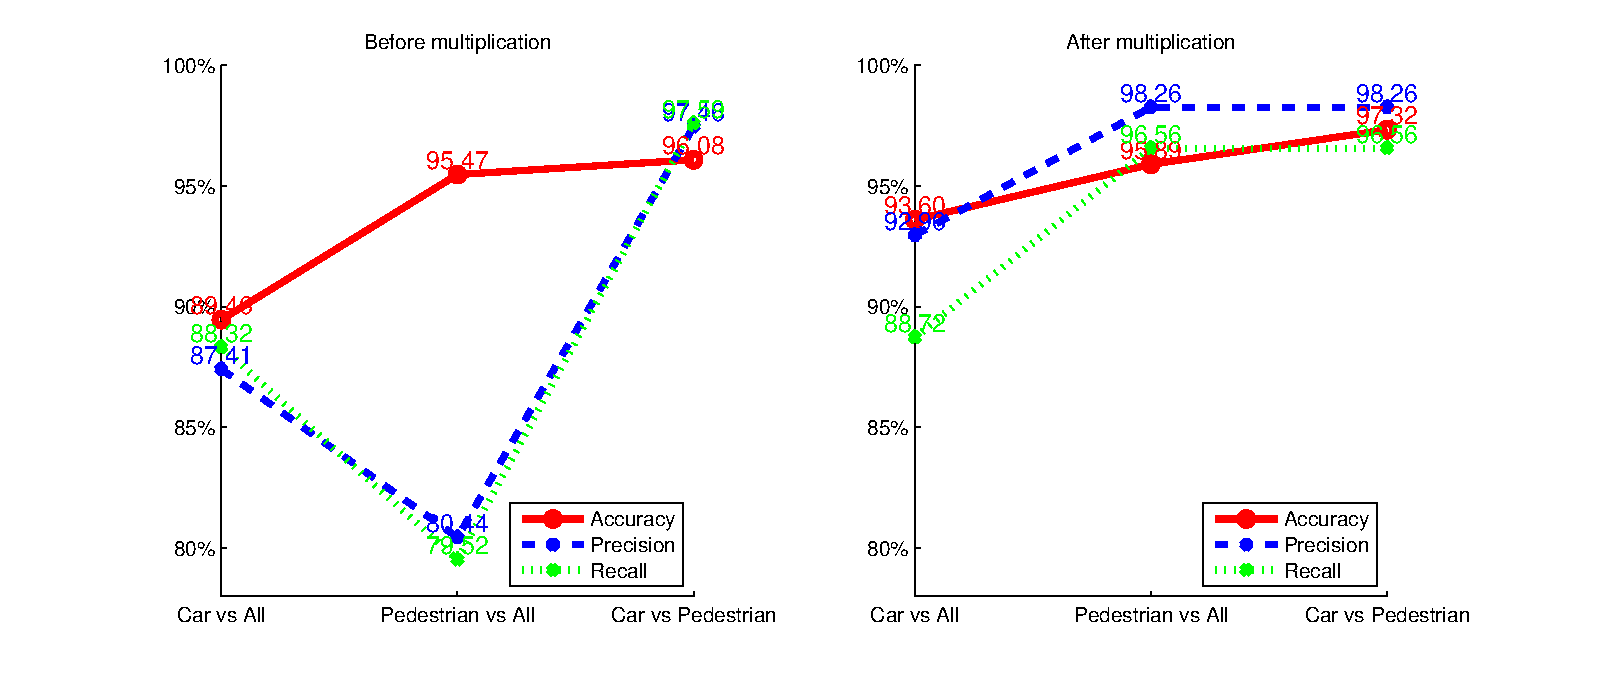
\includegraphics[width=.9\textwidth]{test_apr.eps}
%\fbox{\rule[-.5cm]{0cm}{4cm} \rule[-.5cm]{4cm}{0cm}}
\end{center}
\caption{Accuracy, precision, and recall rate of the 3 classifiers (Car vs All, Pedestrian vs All, and Car vs Pedestrian) on the object recognition task before and after the image multiplication.
\label{fig:test-apr}}
\end{figure}


From Figure \ref{fig:test-apr}, we can conclude that multiplying images will also increase the accuracy, precision, and recall rate. Using $43536$ positive samples and $20000$ negative samples, we obtain a precision rate range from $92.96\%$ to $98.26\%$ and a recall rate range from $88.72\%$ to $96.56\%$. It is reasonable to consider that if we collect more training data or multiply more images with existing data, we will be able to get better performance. But that will also leads to more expensive training and testing cost. Anyway, we observe a good performance of Selective Search + SVM on the object recognition task.

\begin{figure}[htb]
\begin{center}
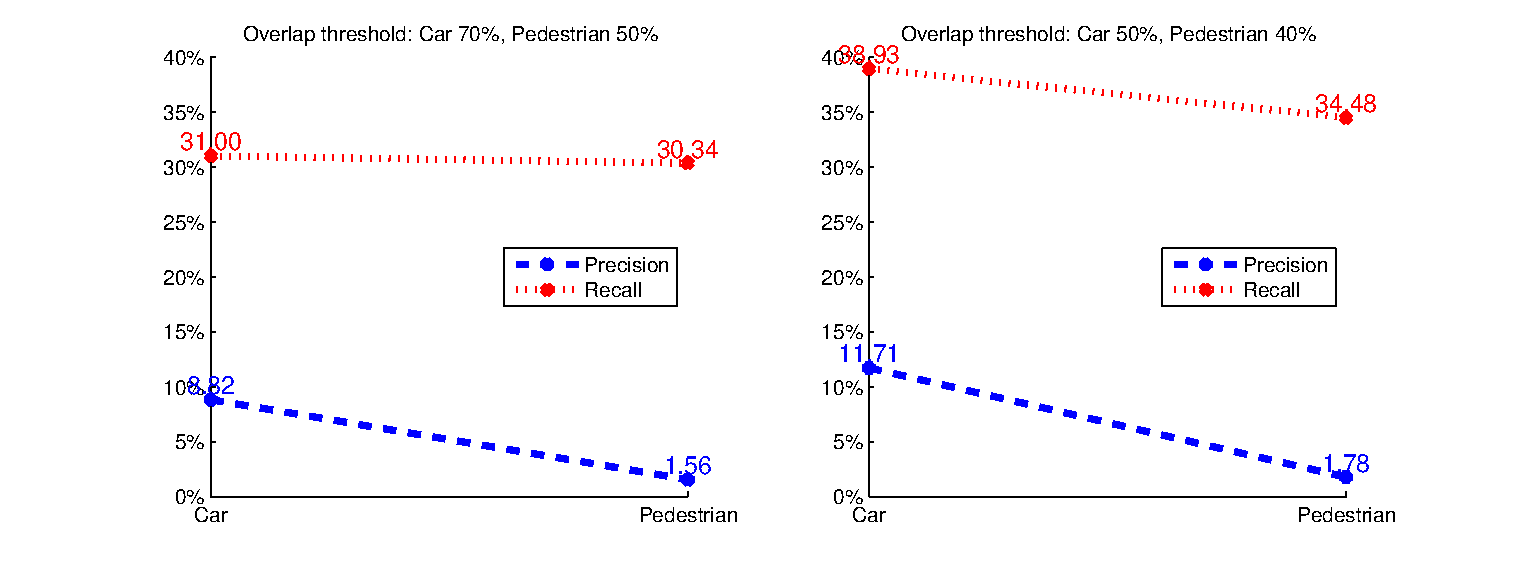
\includegraphics[width=\textwidth]{test-result.eps}
\end{center}
\caption{Precision and recall rate of the 2 classes (car and pedestrian) on the final object detection task. Left: results when the overlap threshold is $70\%$ for cars and $50\%$ for pedestrians. Right: results when the overlap threshold is $50\%$ for cars and $40\%$ for pedestrians
\label{fig:test-result}}
\end{figure}

\begin{table}[htb]
\caption{Comparison of performance on object recognition task and object detection task}
\label{tab:comp}
\begin{center}
\begin{tabular}{lcc}
\multicolumn{1}{c}{} &\multicolumn{1}{c}{\bf Object recognition}  &\multicolumn{1}{c}{\bf Object detection}
\\ \hline \\
Average precision rate & $96.50\%$ & $5.19\%$ \\
Average recall rate    & $93.95\%$ & $30.67\%$ \\
\end{tabular}
\end{center}
\end{table}

However, on the real test set, the precision and recall rate in Figure \ref{fig:test-result} is very low compared to the testing result on the object recognition task in Figure \ref{fig:test-apr}. The average performance is compared in Table \ref{tab:comp}. We try to analyze our false results from two aspects: false positive results and false negative results.

\begin{figure}[htb]
\begin{subfigure}[b]{0.5\textwidth}
    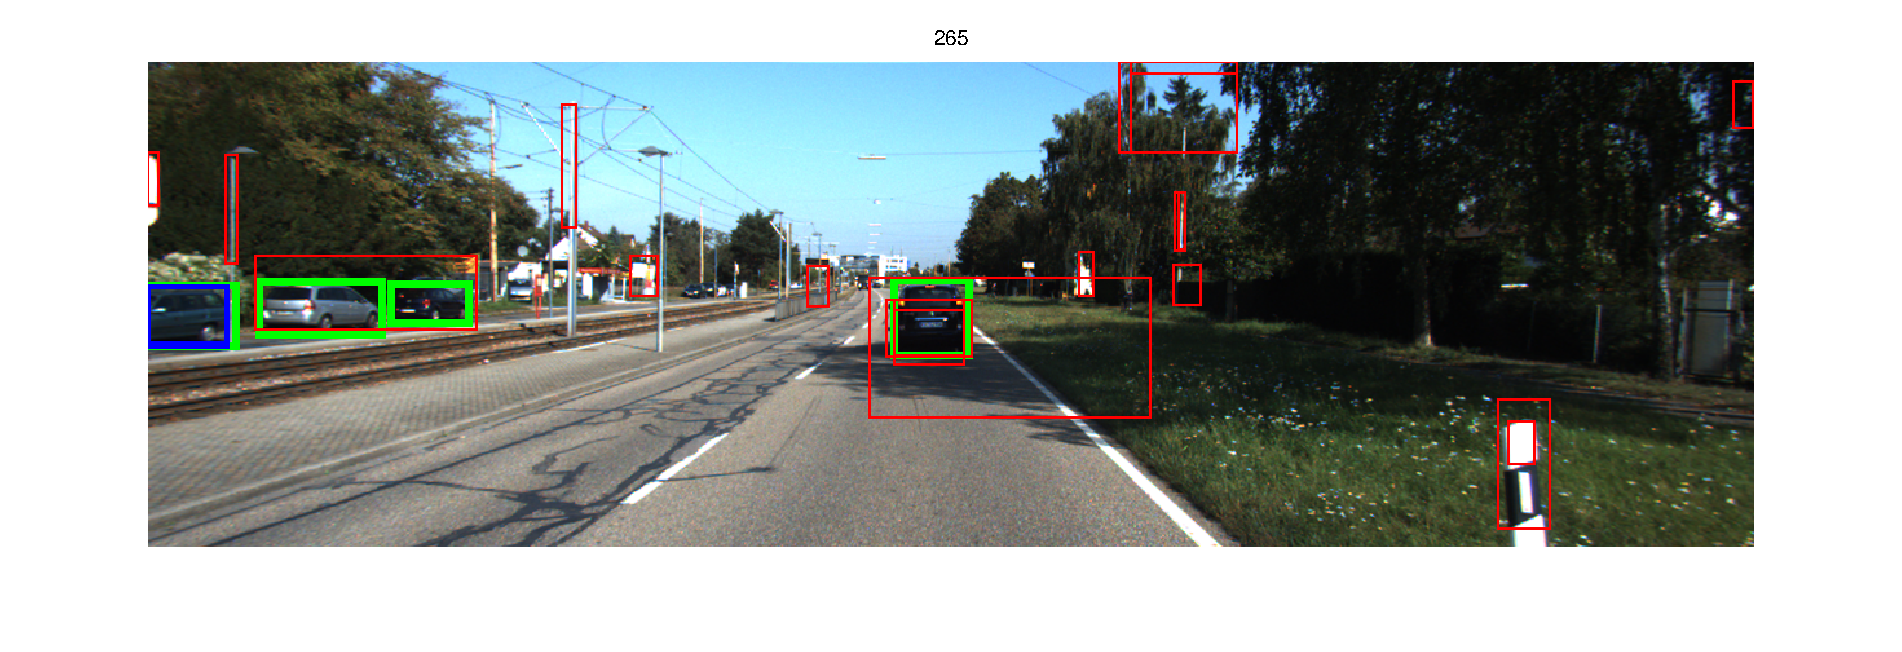
\includegraphics[width=.9\textwidth]{test-fp1.eps}
    \label{fig:test-fp1}
\end{subfigure}
\begin{subfigure}[b]{0.5\textwidth}
    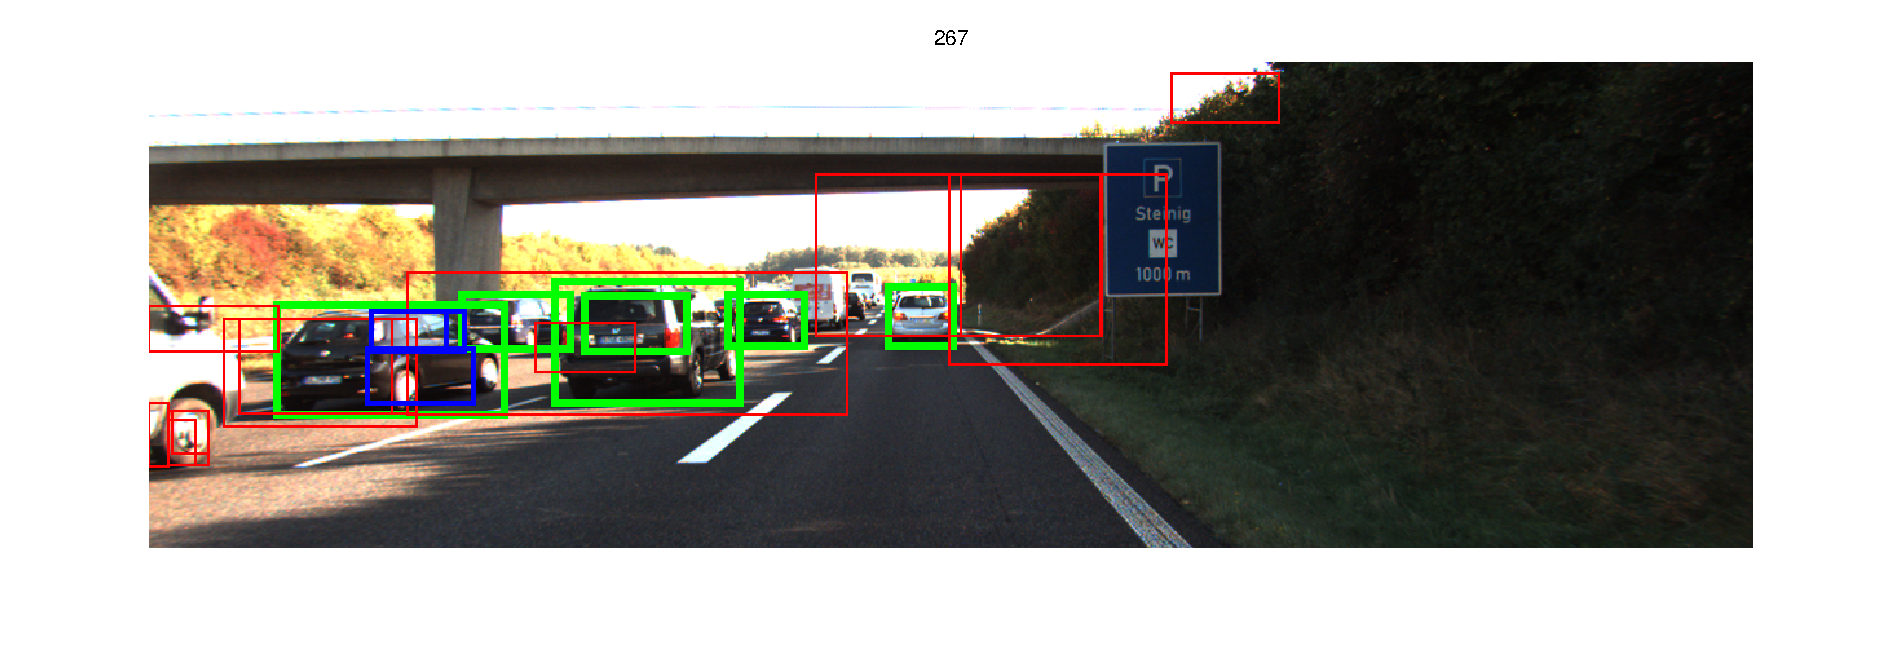
\includegraphics[width=.9\textwidth]{test-fp2.eps}
    \label{fig:test-fp2}
\end{subfigure}

\begin{subfigure}[b]{0.5\textwidth}
    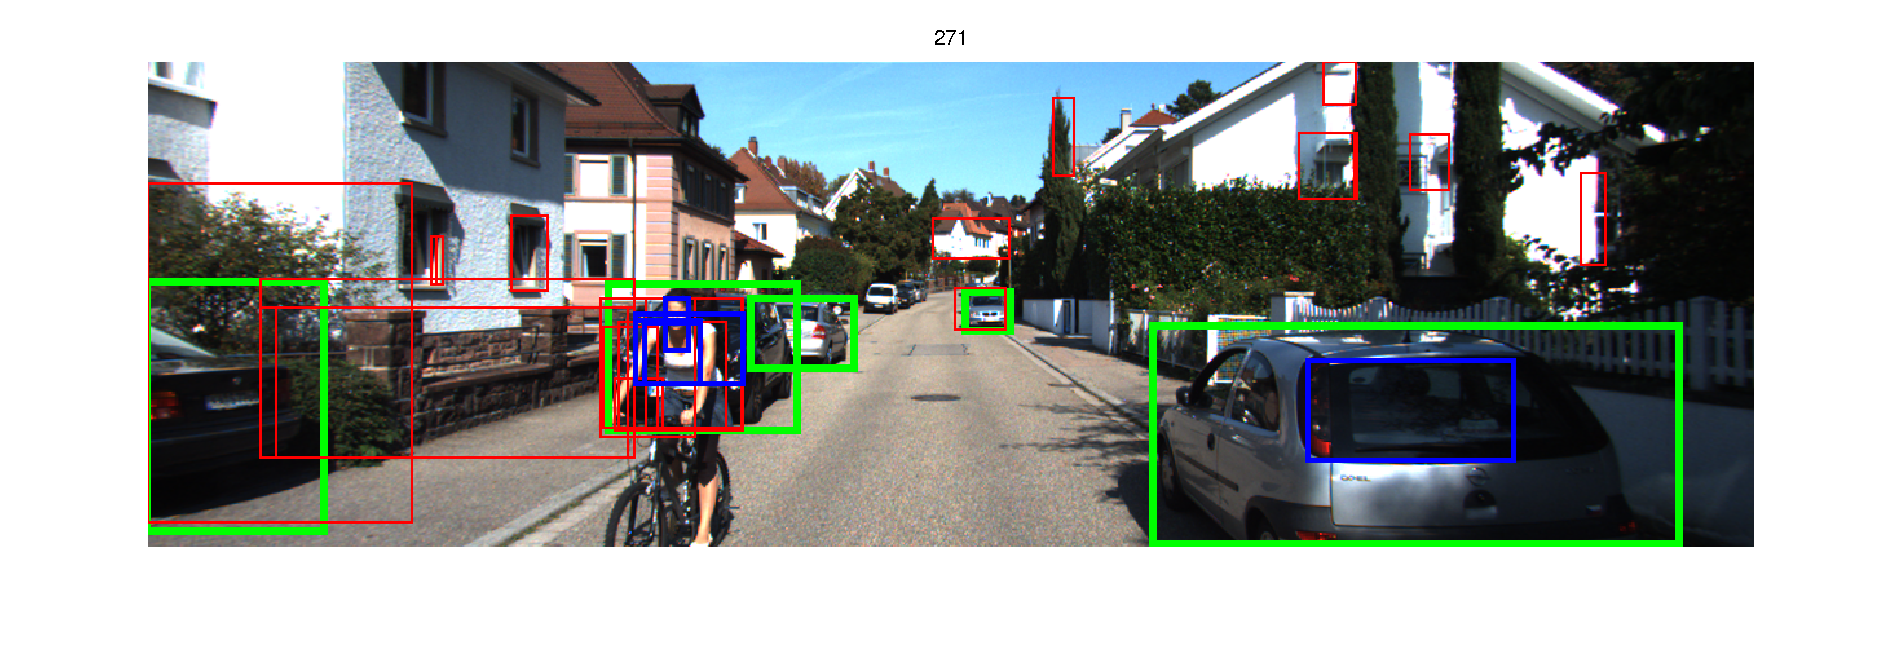
\includegraphics[width=.9\textwidth]{test-fp3.eps}
    \label{fig:test-fp3}
\end{subfigure}
\begin{subfigure}[b]{0.5\textwidth}
    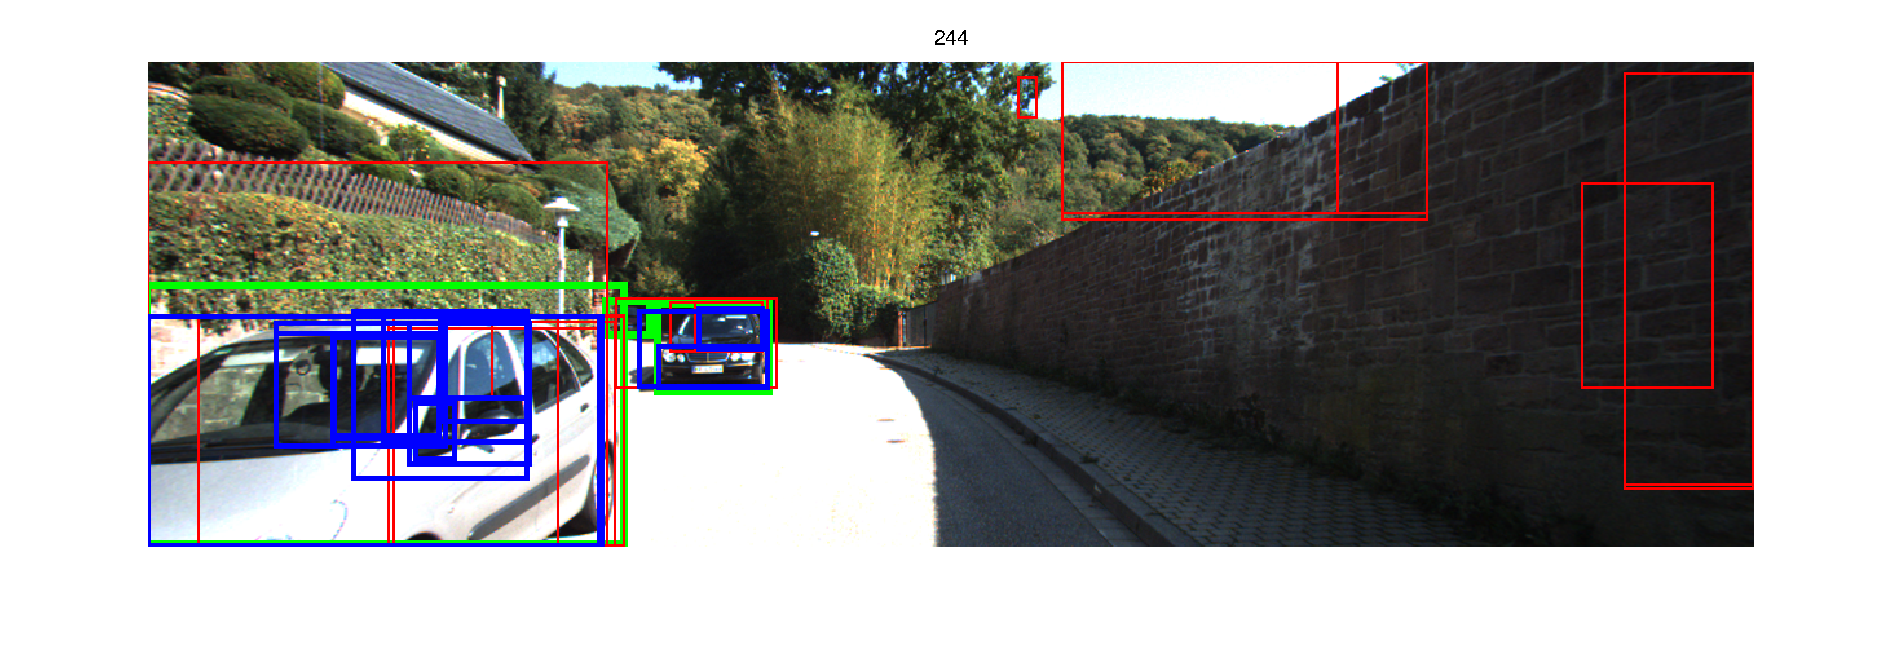
\includegraphics[width=.9\textwidth]{test-fp4.eps}
    \label{fig:test-fp4}
\end{subfigure}
\caption{False Positive results. The green thick bounding box is the ground truth, the blue moderate bounding box is relevant output, and the red thin bounding box is the false positive output. In these cases, most of the cars and pedestrians are classified successfully, but some background segments, such as the road signs, are also classified as cars (or pedestrians).
\label{fig:test-fp}}
\end{figure}

On the one hand, we can analyze the false positive results from Figure \ref{fig:test-fp}. We notice that the detector find out most of the cars and pedestrians, while it also put extra bounding box on the background wall or the traffic sign. This problem also indicates the difficulty in training the negative samples, since they are harder to cluster, and full of different textures. And if we simply add more negative samples, then the negative output will dominate the classifier. In addition, Selective Search is a general image segmentation algorithm, so it need to be modified and trained to better fit this road object detection task. 

\begin{figure}[htb]
\begin{subfigure}[b]{0.5\textwidth}
    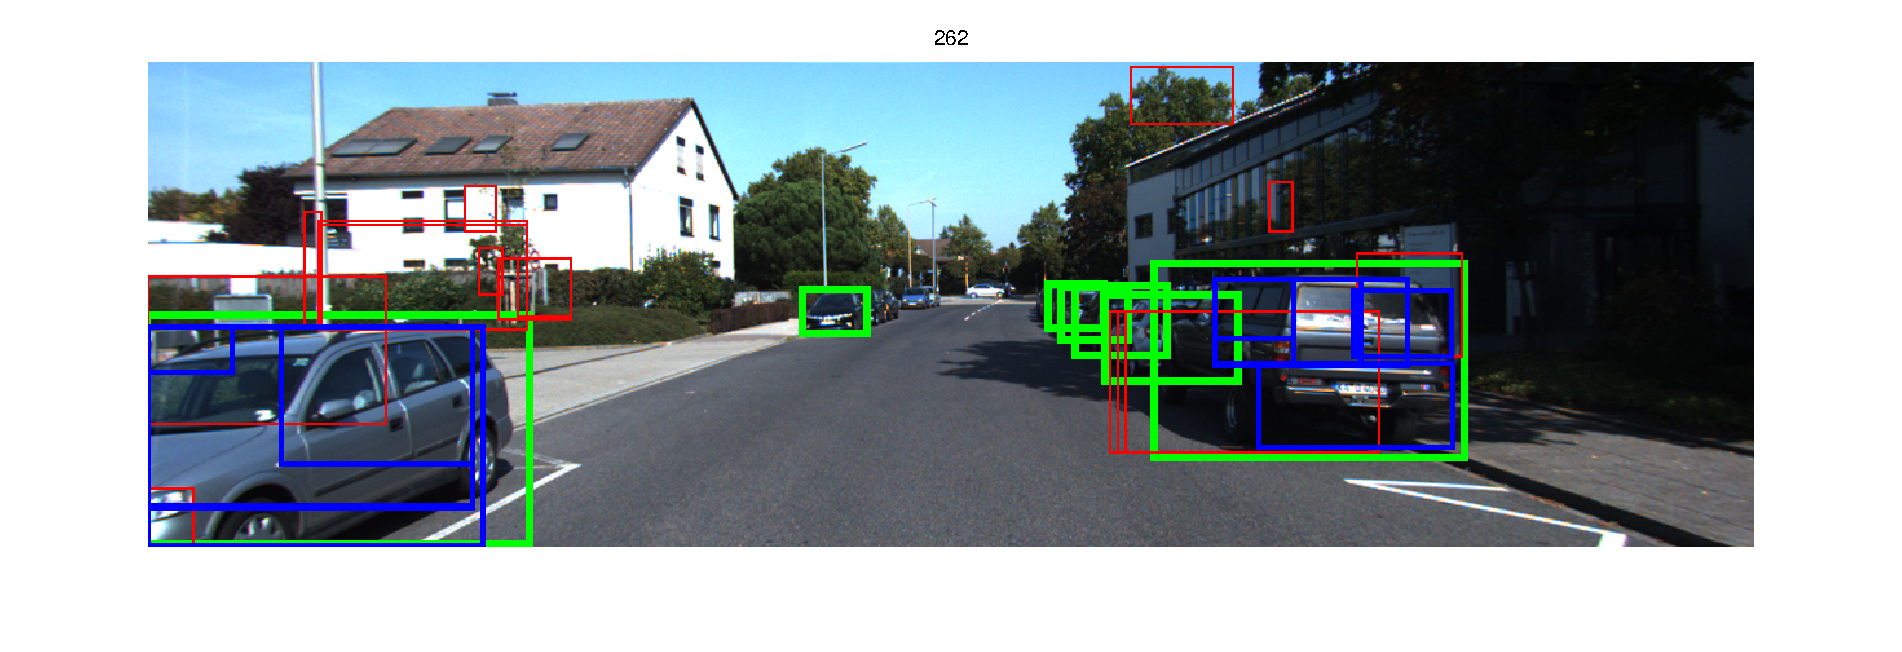
\includegraphics[width=.9\textwidth]{test-fn1.eps}
    \label{fig:test-fn1}
\end{subfigure}
\begin{subfigure}[b]{0.5\textwidth}
    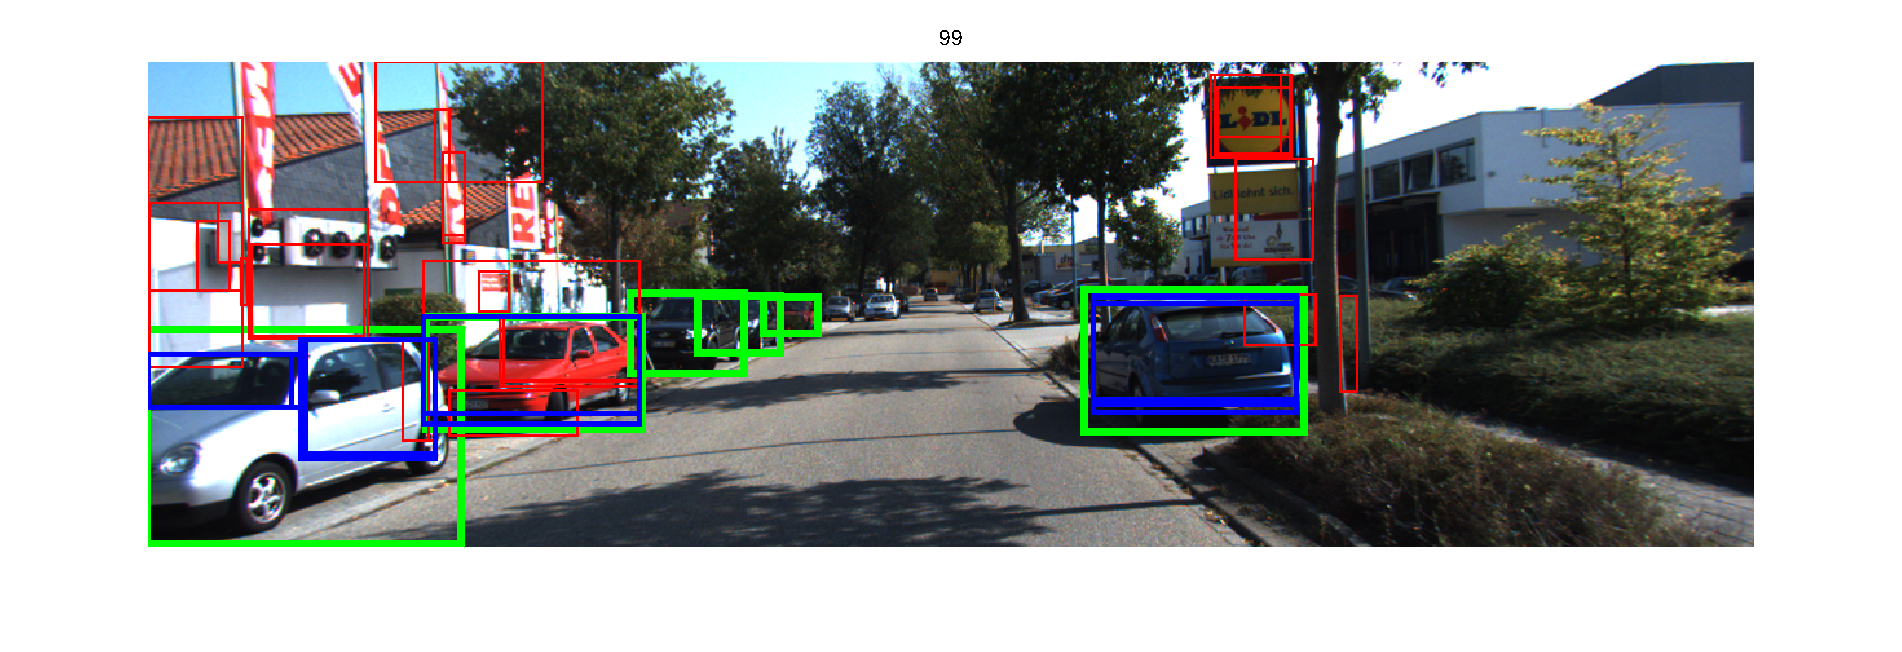
\includegraphics[width=.9\textwidth]{test-fn2.eps}
    \label{fig:test-fn2}
\end{subfigure}

\begin{subfigure}[b]{0.5\textwidth}
    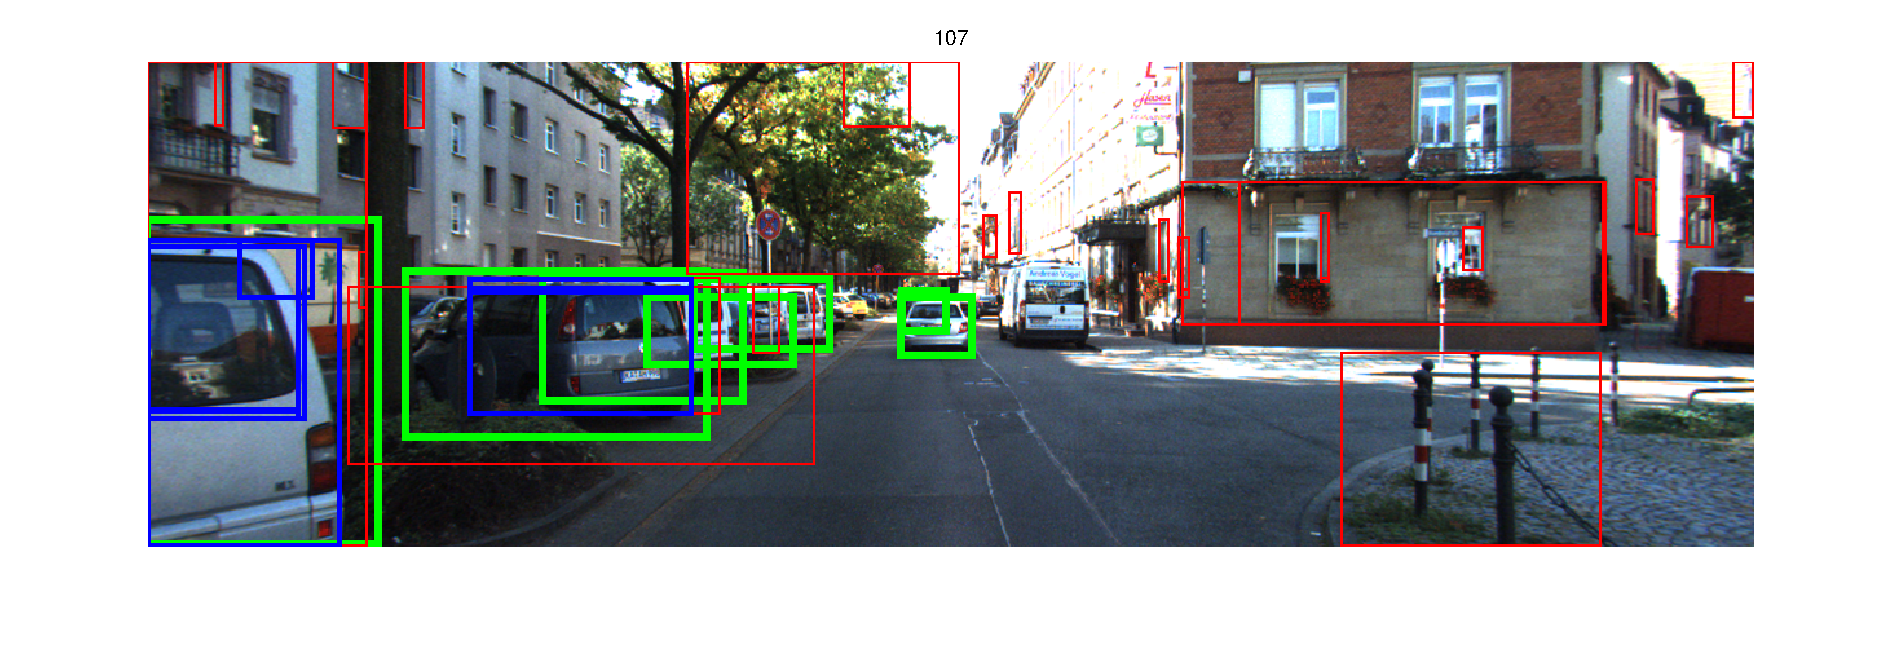
\includegraphics[width=.9\textwidth]{test-fn3.eps}
    \label{fig:test-fn3}
\end{subfigure}
\begin{subfigure}[b]{0.5\textwidth}
    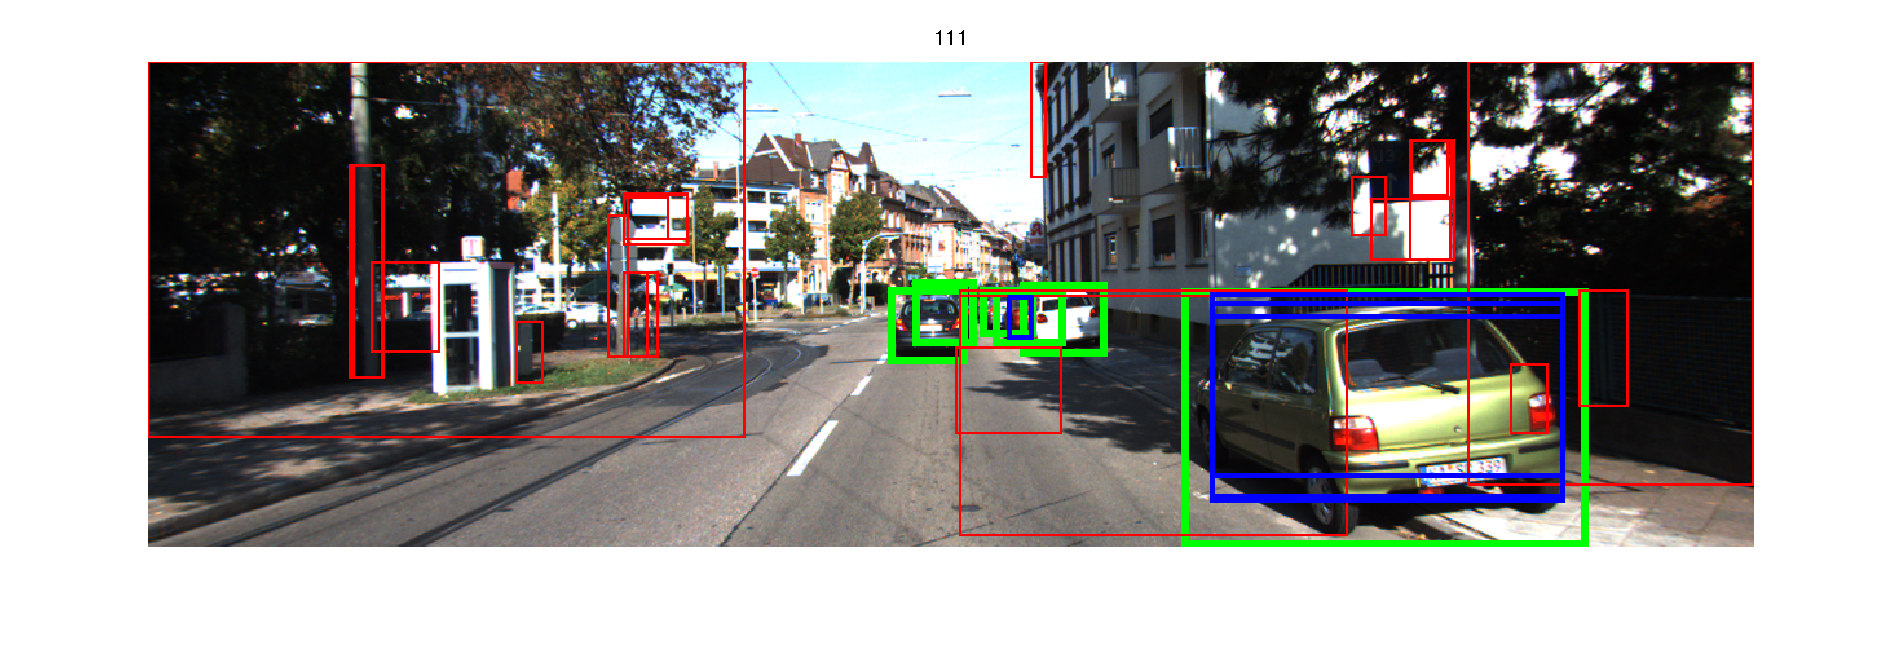
\includegraphics[width=.9\textwidth]{test-fn4.eps}
    \label{fig:test-fn4}
\end{subfigure}
\caption{False Negative results. The green thick bounding box is the ground truth, the blue moderate bounding box is relevant output, and the red thin bounding box is the false positive output. In these cases, most of the cars and pedestrians that close to the observer are classified successfully, but those objects that far away from the observer are not found.
\label{fig:test-fn}}
\end{figure}

On the other hand, there are many false negative results when the objects are small, as shown in Figure \ref{fig:test-fn}. We can observe from Figure \ref{fig:test-fn} that the proposals are relatively big compared to the small cars. However, if we decrease the expected size of bounding box, we will miss the big car that close to the observer. An alternative way to do this is trying multiple times with different segment sizes, and then merge the boxes based on similarity. We try to do this trick, but the running time is not affordable. 

\subsection{Regionlets feature boosting}

The training of the classifiers for regionlets features is described in Section \ref{training_regionlets}. Since we use one-split decision tree as the weak classifier, the classifiers we get is binary. We again trained 3 classifiers: (1) Car vs All, (2) Pedestrian vs All, and (3) Car vs Pedestrian. We used Gentle Adaboost Algorithm[] to get boosted classifiers. The training set is preprocessed in the same way as SVM. 

\subsection{CNN}

We try to employ a binary classifier with CNN using the DeepLearnToolbox \cite{palm2012prediction}. We train and test a $6C-2S-12C-2S$ CNN on the MNIST Database \cite{lecun1998gradient}, and we got a $11.13\%$ error rate after 1 epoch, and it will drop to $4.56\%$ after 5 epochs. However, it cannot even work with the object recognition task. We tried different parameters and structers of the CNN, but it does not perform well even on the cropped images. It is hard to tune the structure of the CNN based on the cross validation, and the sample code for MNIST should be modified carefully to fit this project.

\section{Conclusion}

From our experiment results in Table \ref{tab:comp}, our project performs well on the object recognition task (average $precision=96.50\%, recall=93.95\%$), but performs terrible on the object detection task (average $precision=5.19\%, recall=30.67\%$). The object recognition task used the cropped images to train and test, while the real road images are more complicated, more truncated, and of different scales.

In the future, we could run the code on GPU to speed up. There are many limitations of our work which can be improved by parallelize the code on GPU. For example, it will help to iteratively add more false positive samples to the retrain procedure in a short time. It will also be helpful if we want to combine several different classifier together and output a weighted result.

What's more, in order to get more training sets with different features, we could use some pedestrian data sets in the future, including Caltech Pedestrian Detection Benchmark \cite{Dollar2009} and Daimler Pedestrian Segmentation Benchmark Data Set \cite{flohr2013pedcut}. The Caltech Pedestrian data set also includes sequential image flow generated from street view videos, which will contribute to the utilization of context information for autonomous driving. 

Generally speaking, each of us had fun in this course project, and we learned some first hand experience by trying different techniques and solve unexpected problems. Since we are still interested in this field, we will take CSC2523 and CSC2541 respectively, continue working on this topic.


\iffalse 

\sectinnnnnon{Submission of papers to NIPS 2015}

NIPS requires electronic submissions.  The electronic submission site is  
\begin{center}
   \url{http://papers.nips.cc}
\end{center}

Please read carefully the
instructions below, and follow them faithfully.
\subsection{Style}

Papers to be submitted to NIPS 2015 must be prepared according to the
instructions presented here. Papers may be only up to eight pages long,
including figures. Since 2009 an additional ninth page \textit{containing only
cited references} is allowed. Papers that exceed nine pages will not be
reviewed, or in any other way considered for presentation at the conference.
%This is a strict upper bound. 

Please note that this year we have introduced automatic line number generation
into the style file (for \LaTeXe and Word versions). This is to help reviewers
refer to specific lines of the paper when they make their comments. Please do
NOT refer to these line numbers in your paper as they will be removed from the
style file for the final version of accepted papers.

The margins in 2015 are the same as since 2007, which allow for $\approx 15\%$
more words in the paper compared to earlier years. We are also again using 
double-blind reviewing. Both of these require the use of new style files.

Authors are required to use the NIPS \LaTeX{} style files obtainable at the
NIPS website as indicated below. Please make sure you use the current files and
not previous versions. Tweaking the style files may be grounds for rejection.

%% \subsection{Double-blind reviewing}

%% This year we are doing double-blind reviewing: the reviewers will not know 
%% who the authors of the paper are. For submission, the NIPS style file will 
%% automatically anonymize the author list at the beginning of the paper.

%% Please write your paper in such a way to preserve anonymity. Refer to
%% previous work by the author(s) in the third person, rather than first
%% person. Do not provide Web links to supporting material at an identifiable
%% web site.

%%\subsection{Electronic submission}
%%
%% \textbf{THE SUBMISSION DEADLINE IS June 5, 2015. SUBMISSIONS MUST BE LOGGED BY
%% 23:00, June 5, 2015, UNIVERSAL TIME}

%% You must enter your submission in the electronic submission form available at
%% the NIPS website listed above. You will be asked to enter paper title, name of
%% all authors, keyword(s), and data about the contact
%% author (name, full address, telephone, fax, and email). You will need to
%% upload an electronic (postscript or pdf) version of your paper.

%% You can upload more than one version of your paper, until the
%% submission deadline. We strongly recommended uploading your paper in
%% advance of the deadline, so you can avoid last-minute server congestion.
%%
%% Note that your submission is only valid if you get an e-mail
%% confirmation from the server. If you do not get such an e-mail, please
%% try uploading again. 


\subsection{Retrieval of style files}

The style files for NIPS and other conference information are available on the World Wide Web at
\begin{center}
   \url{http://www.nips.cc/}
\end{center}
The file \verb+nips2015.pdf+ contains these 
instructions and illustrates the
various formatting requirements your NIPS paper must satisfy. \LaTeX{}
users can choose between two style files:
\verb+nips15submit_09.sty+ (to be used with \LaTeX{} version 2.09) and
\verb+nips15submit_e.sty+ (to be used with \LaTeX{}2e). The file
\verb+nips2015.tex+ may be used as a ``shell'' for writing your paper. All you
have to do is replace the author, title, abstract, and text of the paper with
your own. The file
\verb+nips2015.rtf+ is provided as a shell for MS Word users.

The formatting instructions contained in these style files are summarized in
sections \ref{gen_inst}, \ref{headings}, and \ref{others} below.

%% \subsection{Keywords for paper submission}
%% Your NIPS paper can be submitted with any of the following keywords (more than one keyword is possible for each paper):

%% \begin{verbatim}
%% Bioinformatics
%% Biological Vision
%% Brain Imaging and Brain Computer Interfacing
%% Clustering
%% Cognitive Science
%% Control and Reinforcement Learning
%% Dimensionality Reduction and Manifolds
%% Feature Selection
%% Gaussian Processes
%% Graphical Models
%% Hardware Technologies
%% Kernels
%% Learning Theory
%% Machine Vision
%% Margins and Boosting
%% Neural Networks
%% Neuroscience
%% Other Algorithms and Architectures
%% Other Applications
%% Semi-supervised Learning
%% Speech and Signal Processing
%% Text and Language Applications

%% \end{verbatim}

\section{General formatting instructions}
\label{gen_inst}

The text must be confined within a rectangle 5.5~inches (33~picas) wide and
9~inches (54~picas) long. The left margin is 1.5~inch (9~picas).
Use 10~point type with a vertical spacing of 11~points. Times New Roman is the
preferred typeface throughout. Paragraphs are separated by 1/2~line space,
with no indentation.

Paper title is 17~point, initial caps/lower case, bold, centered between
2~horizontal rules. Top rule is 4~points thick and bottom rule is 1~point
thick. Allow 1/4~inch space above and below title to rules. All pages should
start at 1~inch (6~picas) from the top of the page.

%The version of the paper submitted for review should have ``Anonymous Author(s)'' as the author of the paper.

For the final version, authors' names are
set in boldface, and each name is centered above the corresponding
address. The lead author's name is to be listed first (left-most), and
the co-authors' names (if different address) are set to follow. If
there is only one co-author, list both author and co-author side by side.

Please pay special attention to the instructions in section \ref{others}
regarding figures, tables, acknowledgments, and references.

\section{Headings: first level}
\label{headings}

First level headings are lower case (except for first word and proper nouns),
flush left, bold and in point size 12. One line space before the first level
heading and 1/2~line space after the first level heading.

\subsection{Headings: second level}

Second level headings are lower case (except for first word and proper nouns),
flush left, bold and in point size 10. One line space before the second level
heading and 1/2~line space after the second level heading.

\subsubsection{Headings: third level}

Third level headings are lower case (except for first word and proper nouns),
flush left, bold and in point size 10. One line space before the third level
heading and 1/2~line space after the third level heading.

\section{Citations, figures, tables, references}
\label{others}

These instructions apply to everyone, regardless of the formatter being used.

\subsection{Citations within the text}

Citations within the text should be numbered consecutively. The corresponding
number is to appear enclosed in square brackets, such as [1] or [2]-[5]. The
corresponding references are to be listed in the same order at the end of the
paper, in the \textbf{References} section. (Note: the standard
\textsc{Bib\TeX} style \texttt{unsrt} produces this.) As to the format of the
references themselves, any style is acceptable as long as it is used
consistently.

As submission is double blind, refer to your own published work in the 
third person. That is, use ``In the previous work of Jones et al.\ [4]'',
not ``In our previous work [4]''. If you cite your other papers that
are not widely available (e.g.\ a journal paper under review), use
anonymous author names in the citation, e.g.\ an author of the
form ``A.\ Anonymous''. 


\subsection{Footnotes}

Indicate footnotes with a number\footnote{Sample of the first footnote} in the
text. Place the footnotes at the bottom of the page on which they appear.
Precede the footnote with a horizontal rule of 2~inches
(12~picas).\footnote{Sample of the second footnote}

\subsection{Figures}

All artwork must be neat, clean, and legible. Lines should be dark
enough for purposes of reproduction; art work should not be
hand-drawn. The figure number and caption always appear after the
figure. Place one line space before the figure caption, and one line
space after the figure. The figure caption is lower case (except for
first word and proper nouns); figures are numbered consecutively.

Make sure the figure caption does not get separated from the figure.
Leave sufficient space to avoid splitting the figure and figure caption.

You may use color figures. 
However, it is best for the
figure captions and the paper body to make sense if the paper is printed
either in black/white or in color.
\begin{figure}[h]
\begin{center}
%\framebox[4.0in]{$\;$}
\fbox{\rule[-.5cm]{0cm}{4cm} \rule[-.5cm]{4cm}{0cm}}
\end{center}
\caption{Sample figure caption.}
\end{figure}

\subsection{Tables}

All tables must be centered, neat, clean and legible. Do not use hand-drawn
tables. The table number and title always appear before the table. See
Table~\ref{sample-table}.

Place one line space before the table title, one line space after the table
title, and one line space after the table. The table title must be lower case
(except for first word and proper nouns); tables are numbered consecutively.

\begin{table}[t]
\caption{Sample table title}
\label{sample-table}
\begin{center}
\begin{tabular}{ll}
\multicolumn{1}{c}{\bf PART}  &\multicolumn{1}{c}{\bf DESCRIPTION}
\\ \hline \\
Dendrite         &Input terminal \\
Axon             &Output terminal \\
Soma             &Cell body (contains cell nucleus) \\
\end{tabular}
\end{center}
\end{table}

\section{Final instructions}
Do not change any aspects of the formatting parameters in the style files.
In particular, do not modify the width or length of the rectangle the text
should fit into, and do not change font sizes (except perhaps in the
\textbf{References} section; see below). Please note that pages should be
numbered.

\section{Preparing PostScript or PDF files}

Please prepare PostScript or PDF files with paper size ``US Letter'', and
not, for example, ``A4''. The -t
letter option on dvips will produce US Letter files.

Fonts were the main cause of problems in the past years. Your PDF file must
only contain Type 1 or Embedded TrueType fonts. Here are a few instructions
to achieve this.

\begin{itemize}

\item You can check which fonts a PDF files uses.  In Acrobat Reader,
select the menu Files$>$Document Properties$>$Fonts and select Show All Fonts. You can
also use the program \verb+pdffonts+ which comes with \verb+xpdf+ and is
available out-of-the-box on most Linux machines.

\item The IEEE has recommendations for generating PDF files whose fonts
are also acceptable for NIPS. Please see
\url{http://www.emfield.org/icuwb2010/downloads/IEEE-PDF-SpecV32.pdf}

\item LaTeX users:

\begin{itemize}

\item Consider directly generating PDF files using \verb+pdflatex+
(especially if you are a MiKTeX user). 
PDF figures must be substituted for EPS figures, however.

\item Otherwise, please generate your PostScript and PDF files with the following commands:
\begin{verbatim} 
dvips mypaper.dvi -t letter -Ppdf -G0 -o mypaper.ps
ps2pdf mypaper.ps mypaper.pdf
\end{verbatim}

Check that the PDF files only contains Type 1 fonts. 
%For the final version, please send us both the Postscript file and
%the PDF file. 

\item xfig "patterned" shapes are implemented with 
bitmap fonts.  Use "solid" shapes instead. 
\item The \verb+\bbold+ package almost always uses bitmap
fonts.  You can try the equivalent AMS Fonts with command
\begin{verbatim}
\usepackage[psamsfonts]{amssymb}
\end{verbatim}
 or use the following workaround for reals, natural and complex: 
\begin{verbatim}
\newcommand{\RR}{I\!\!R} %real numbers
\newcommand{\Nat}{I\!\!N} %natural numbers 
\newcommand{\CC}{I\!\!\!\!C} %complex numbers
\end{verbatim}

\item Sometimes the problematic fonts are used in figures
included in LaTeX files. The ghostscript program \verb+eps2eps+ is the simplest
way to clean such figures. For black and white figures, slightly better
results can be achieved with program \verb+potrace+.
\end{itemize}
\item MSWord and Windows users (via PDF file):
\begin{itemize}
\item Install the Microsoft Save as PDF Office 2007 Add-in from
\url{http://www.microsoft.com/downloads/details.aspx?displaylang=en\&familyid=4d951911-3e7e-4ae6-b059-a2e79ed87041}
\item Select ``Save or Publish to PDF'' from the Office or File menu
\end{itemize}
\item MSWord and Mac OS X users (via PDF file):
\begin{itemize}
\item From the print menu, click the PDF drop-down box, and select ``Save
as PDF...''
\end{itemize}
\item MSWord and Windows users (via PS file):
\begin{itemize}
\item To create a new printer
on your computer, install the AdobePS printer driver and the Adobe Distiller PPD file from
\url{http://www.adobe.com/support/downloads/detail.jsp?ftpID=204} {\it Note:} You must reboot your PC after installing the
AdobePS driver for it to take effect.
\item To produce the ps file, select ``Print'' from the MS app, choose
the installed AdobePS printer, click on ``Properties'', click on ``Advanced.''
\item Set ``TrueType Font'' to be ``Download as Softfont''
\item Open the ``PostScript Options'' folder
\item Select ``PostScript Output Option'' to be ``Optimize for Portability''
\item Select ``TrueType Font Download Option'' to be ``Outline''
\item Select ``Send PostScript Error Handler'' to be ``No''
\item Click ``OK'' three times, print your file.
\item Now, use Adobe Acrobat Distiller or ps2pdf to create a PDF file from
the PS file. In Acrobat, check the option ``Embed all fonts'' if
applicable.
\end{itemize}

\end{itemize}
If your file contains Type 3 fonts or non embedded TrueType fonts, we will
ask you to fix it. 

\subsection{Margins in LaTeX}
 
Most of the margin problems come from figures positioned by hand using
\verb+\special+ or other commands. We suggest using the command
\verb+\includegraphics+
from the graphicx package. Always specify the figure width as a multiple of
the line width as in the example below using .eps graphics
\begin{verbatim}
   \usepackage[dvips]{graphicx} ... 
   \includegraphics[width=0.8\linewidth]{myfile.eps} 
\end{verbatim}
or % Apr 2009 addition
\begin{verbatim}
   \usepackage[pdftex]{graphicx} ... 
   \includegraphics[width=0.8\linewidth]{myfile.pdf} 
\end{verbatim}
for .pdf graphics. 
See section 4.4 in the graphics bundle documentation (\url{http://www.ctan.org/tex-archive/macros/latex/required/graphics/grfguide.ps}) 
 
A number of width problems arise when LaTeX cannot properly hyphenate a
line. Please give LaTeX hyphenation hints using the \verb+\-+ command.


\subsubsection*{Acknowledgments}

Use unnumbered third level headings for the acknowledgments. All
acknowledgments go at the end of the paper. Do not include 
acknowledgments in the anonymized submission, only in the 
final paper. 

\fi 

\bibliographystyle{IEEEtran}
\bibliography{ref}

\iffalse
References follow the acknowledgments. Use unnumbered third level heading for
the references. Any choice of citation style is acceptable as long as you are
consistent. It is permissible to reduce the font size to `small' (9-point) 
when listing the references. {\bf Remember that this year you can use
a ninth page as long as it contains \emph{only} cited references.}
\fi 

\end{document}
